% Copyright 2007 by Till Tantau

%
% This file may be distributed and/or modified
%
% 1. under the LaTeX Project Public License and/or
% 2. under the GNU Public License.
%
% See the file doc/licenses/LICENSE for more details.


\lecture[12]{Power and false positives}{lecture-text}

\subtitle{hypothesis testing, and one-sided tests}

\date{13 October 2015}

% pp. 218-(242?)


\begin{document}

\begin{frame}
  \maketitle
\end{frame}

%%%%%
\begin{frame}{Last time}

  \begin{itemize}
    \item \structure{Null hypothesis, $H_0$:} ``what if this was just random noise?''
    \item \structure{$P$-value:} the probability of seeing something as suprising as we did, if that was true.
    \item the $t$-test: 
      \begin{itemize}
        \item ``The sample means differ, but could the population means be the same?''
        \item $t_s = (\bar y_1 - \bar y_2) / \SE_{\bar Y_1 - \bar Y_2}$
        \item also need: degrees of freedom.
      \end{itemize}
    \item \structure{Significance value:} $\alpha$, the cutoff for ``good evidence against $H_0$.''
  \end{itemize}

\end{frame}


\begin{frame}\frametitle<presentation>{Outline}
  \tableofcontents
\end{frame}



\section{Hypothesis testing}


\subsection{False positive rates}
%%%%%
\begin{frame}{Interpretation of $\alpha$}

    Wait, what is $\alpha$?

  \vspace{2em}
  \pause

  It is the \alert{cutoff} for ``statistically significant evidence''
  for the $P$-value.

    \vspace{2em}

    More concretely, it is the 
  \begin{block}{False positive rate:}
    If we did the experiment many times,\\
    \structure{and there was no real effect} ($H_0$ is true)\\
    how often would we \alert{wrongly} conclude there is an effect?
  \end{block}

  \pause
    \vspace{2em}
    \structure{Only applies} if there is \alert{no} real effect.

\end{frame}



%%%%%
\begin{frame}{Example: Music and Marigolds}

    Suppose many researchers run experiments\\
    to test whether marigolds grow taller \\
    when listening to Bach (mean height $\mu_1$) \\
    or Mozart (mean height $\mu_2$). 


    \vspace{2em}

    \begin{align*}
        H_0 &: \quad \mu_1 = \mu_2  \\
        H_A &: \quad \mu_1 \neq \mu_2 
    \end{align*}

    \vspace{2em}

    If everyone uses $\alpha=0.05$ then
    \begin{itemize}
        \item 95\% would find no significant effect
        \item 2.5\% would find statistically significant evidence that Mozart is better
        \item 2.5\% would find statistically significant evidence that Bach is better
    \end{itemize}

\end{frame}

%%%%%
\begin{frame}{Why is $\alpha$ always 5\%?}

    \begin{center}
        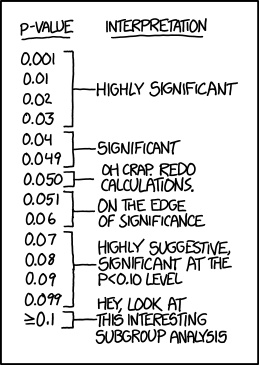
\includegraphics[width=0.6\textwidth]{p_values}
        \figcaption{xkcd:1478}
    \end{center}

\end{frame}



%%%%%
\begin{frame}{Are 90\% of all studies false?}

        (No.)

    \vspace{2em}
    \pause

    \begin{quote}
        \small
        Suppose you throw a dart at the Big Chart O' Human Metabolic Pathways and supplement your experimental group with the chemical you hit. Then ten years later you come back and see how many of them died of heart attacks.
        Most chemicals on the Big Chart probably don't prevent heart attacks. Let's say only one in a thousand do. 
    \end{quote}

    \vspace{1em}

    If only studies significant at $\alpha=5\%$ publish,
    what proportion are wrong?

    \vspace{1em}
        
    \begin{quote}
        \pause Maybe your study will successfully find that 1/1000. But the 999 inactive chemicals will also throw up about 50 (999 $\times$ 5\%) false positives significant at the 5\% level. Therefore, even if you conduct your study perfectly, and it shows a significant decrease in heart attacks, there's about a 98\% chance it's false.
    \end{quote}
    \figcaption{http://slatestarcodex.com/2013/02/17/90-of-all-claims-about-the-problems-with-medical-studies-are-wrong/}


\end{frame}

%%%%%%%
\begin{frame}{Wait, why aren't 90\% of studies false?}
        \begin{quote}
    When doctors say that, for example, iron supplements help anaemia, it's not because they hit iron on their Big Chart O' Human Metabolic Pathways, then ran a single study, got $p = .05$, and rushed off to publish a medical textbook. It's because they knew hemoglobin had iron in it, there are at least 21 randomized controlled studies, probably some had p-values closer to .001 than to .05 even though I don't have any of them in front of me to check, and eventually some really really smart statisticians at the Cochrane Collaboration gave it their seal of approval. 
    \end{quote}
    \figcaption{http://slatestarcodex.com/2013/02/17/90-of-all-claims-about-the-problems-with-medical-studies-are-wrong/}

\end{frame}
%%%%% %%%%%
\section{Type I and Type II Errors}


%%%%%
\begin{frame}{Significance level}

    The \structure{significance level} $\alpha$ is chosen so
    \[
        \prob \{ \text{significant evidence for $H_A$} | \text{$H_0$ is true} \} = \alpha .
    \]
    This is the probability of a \alert{Type I error}.


    \vspace{2em}

    \begin{tabular}{r|cc}
        & \multicolumn{2}{c}{truth} \\
        & $H_0$ & $H_A$ \\
        \hline
        no evidence for $H_A$ & correct & Type II error \\
        good evidence for $H_A$ & Type I error & correct \\
    \end{tabular}

    \vspace{2em}

    \begin{description}
        \item[Type I:] Our significant result is actually due to random noise.
        \item[Type II:] There's something really happening, but we couldn't distinguish it from random noise.
    \end{description}

\end{frame}

%%%%%
\begin{frame}{History and etymology}

  (from: \textit{``The testing of statistical hypotheses in relation to probabilities a priori".} Jerzy Neyman \& Egon Pearson, 1933. )

    \vspace{2em}

  \begin{quote}
    As a result of the statistical analysis we shall decide either
    \begin{itemize}
        \item[(a)] to accept [the hypothesis to be tested,] $H_0$, 
        \item[(b)] to reject $H_0$, 
        \item[(c)] to remain in doubt 
          on the grounds that the evidence provided by the data is inadequate.
    \end{itemize}
    % A statistical test is therefore equivalent to a rule of the following type,
    % \begin{itemize}
    %   \item[(a)] Reject $H_0$ if $\Sigma$ falls into a region $w$.
    %   \item[(b)] Accept $H_0$ if $\Sigma$ falls into another region $w'$.
    %   \item[(c)] Remain in doubt if $\Sigma$ falls into third region $w''$.
    % \end{itemize}
    In making decisions \textit{(a)} or \textit{(b)}
    we shall sometimes be in error
    ... [and] these errors will be of two kinds:
    \begin{itemize}
      \item[(I)] we reject $H_0$ when it is true,
      \item[(II)] we accept $H_0$ when some alternative $H_i$ is true.
    \end{itemize}
    The problem before us is to consider how these errors may be best controlled.
  \end{quote}


\end{frame}

%%%%%
\begin{frame}{Power and Type II error}

    \begin{block}{}
        \alert{Statistical power} is the probability of \emph{not} making a Type II error when $H_A$ is true,
        i.e.\ \structure{of detecting a true signal}.
    \end{block}
    

    \vspace{2em}

    It depends on the \structure{strength} of the signal,\\
    the sample size, and the experimental setup.


    \vspace{2em}

    It does \alert{not} depend on (the random model of) $H_0$.\\
    (but it does depend on the test used)

\end{frame}



%%%%
\section{One--sided $t$-tests}

\subsection{One versus two sides}


%%%%%
\begin{frame}{Back to the $t$ test}


    \begin{center}
        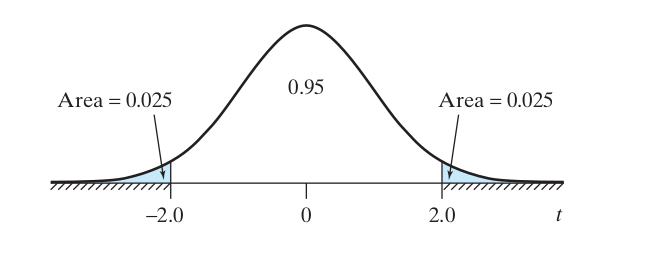
\includegraphics[width=.75\textwidth]{two-tailed-t}
        \flushright \tiny {Samuels, Witmer \& Schaffner}
    \end{center}
    
    If we have an obviously \structure{directional hypothesis}:\\
    we are throwing away power!

    \vspace{2em}

    \structure{The point:} \\
    We want to calibrate our test
    to have \alert{false positive rate} $\alpha=0.05$,
    \ldots but we can still choose such a test to have maximal power \\
    \structure{against our alternative hypothesis}.
\end{frame}

%%%%%%%
\begin{frame}{}

    \centering
    (simulation demonstration)

\end{frame}

%%%%%%%
\begin{frame}{}

    \structure{Example:}
    Measure infection loads in subjects with ($\bar y_1$) and without ($\bar y_2$) a new antibiotic. 

    \vspace{1em}

    \structure{$H_0$:} antibiotic doesn't affect infection load, $\mu_1 = \mu_2$ \\
    \structure{$H_A$:} antibiotic decreases infection load, $\mu_1< \mu_2$ .

\end{frame}


%
\begin{frame}{One or two sides?}

  \begin{description}

    \item[two-sided test:] ``Would the sample means be \alert{this different} if the population means were actually the same?''

    \item[one-sided test:] ``Would this sample mean be \alert{this much larger} than the other if the population means were actually the same?''

  \end{description}

  \vspace{2em}

  \only<1>{
  \structure{More precisely,}
  \begin{description}

    \item[two-sided test:] ``What's the chance that the difference in sample means was at least this large, if the control and treatment populations actually have the same mean?''

    \item[one-sided test:] ``What's the chance that the treatment sample mean is at least this much larger than the control group sample mean,
      if the control and treatment populations actually have the same mean?''

  \end{description}
  }

  \only<2>{
  \structure{More concisely,} with $H_0: \; \mu_1 = \mu_2$:
  \begin{description}

    \item[two-sided test:] $H_A: \; \mu_1 \neq \mu_2$

    \item[one-sided test:] $H_A: \; \mu_1 > \mu_2$

  \end{description}

  \vspace{2em}

  \structure{Note:} can do the test in either direction, replacing "larger" with "smaller".
  }

\end{frame}

%%%
\subsection{Finding a one-sided $P$-value}

\begin{frame}{How to do a one-sided test}

  \begin{center}
  \includegraphicscopyright[width=.8\textwidth]{one-tailed-tests}{Samuels, Whitmer, \& Schaffner}
  \end{center}

  \vspace{-1em}

  \begin{enumerate}
    \item Check if the difference in means is in the right direction. (if not, $P>0.5$).

    \item Compute the $t$ statistic:
      \[
          t_s = \frac{ (\bar y_1 - \bar y_2) - 0}{ \SE_{(\bar Y_1 - \bar Y_2)} }
      \]

    \item Compute the degrees of freedom:
        \[
            df = \frac{ (\SE_1^2 + \SE_2^2)^2 }{ \SE_1^4 / (n_1-1) + \SE_2^4 / (n_2 - 1) }
        \]

    \item Look up the $P$-value. (or, check for significance in Table 4)

  \end{enumerate}


\end{frame}

%%%%%
\begin{frame}{Example: Niacin supplements}

  One group of lambs fed niacin supplements; one control group.  
  \begin{align*}
    H_0 &: \quad \mu_\text{niacin} = \mu_\text{control}  \\
    H_A &: \quad \mu_\text{niacin} > \mu_\text{control}  
  \end{align*}


    \vspace{2em}

  
  Weight gains (lbs):
    \begin{center}
      \begin{tabular}{c|rr}
            & Niacin & Control \\
          \hline
          $\bar y$ & 14 & 10 \\
          $\SE$ & 1.5 & 1.6 \\
     \end{tabular}
   \end{center}
   and $df = 18$.


    \vspace{2em}
    \pause

    \[
    t_s = \frac{ \bar y_\text{niacin} - \bar y_\text{control} }{ \SE_{\bar Y_1 - \bar Y_2} } = \frac{ 14 - 10 }{ \sqrt{ 1.5^2 + 1.6^2 } } = 1.82
    \]
    and $P = 0.043$.
    \pause
    \structure{What would the $P$-value be for a two-sided test?}

\end{frame}


%%
\subsection{What to watch out for}

%
\begin{frame}{How to cheat}

  \begin{enumerate}
    \item Check which mean is larger.
    \item Do a one-sided test, in that direction.
  \end{enumerate}

  \vspace{2em}

  \structure{Solution:} Have a clear hypothesis, that determines the direction beforehand.

  \vspace{2em}

  \begin{block}{Music \& Marigolds}
    If 100 studies look for an effect that isn't real, 
    how many will ``find'' the effect, with
    \begin{itemize}
      \item[\bf (a)] two-sided tests
      \item[\bf (b)] one-sided tests, and a clear prior hypothesis
      \item[\bf (c)] one-sided tests, cheating
    \end{itemize}
  \end{block}

\end{frame}



\section<article>{Summary}
\section<presentation>*{Summary}

\begin{frame}{Summary}
  \begin{enumerate}
    \item $P$-values or confidence intervals: strength of evidence versus effect size
    \item ``Significance level'' can be interpreted as a \alert{false positive rate}
    \item but somehow science moves forward anyhow.
    \item \structure{Type I} error: wrongly interpreting noise as pattern.
    \item \structure{Type II} error: failing to find pattern amidst noise.
    \item \alert{Statistical power} is the chance of finding a true pattern, \\
      or $1-{}$ type II error probability
    \item If the hypothesis is strongly one-sided,
    \item use a one-sided test, which increases power.
    \item But don't cheat.
  \end{enumerate}
\end{frame}

% homework
\begin{frame}{Homework}
  \begin{center}

      7.3.4

    \vspace{2em}

    7.3.5

    \vspace{2em}

    7.5.5

  \end{center}
\end{frame}


\end{document}





